\documentclass{beamer}

\useoutertheme[subsection=false]{miniframes}
\usecolortheme{beaver}
\setbeamertemplate{navigation symbols}{}
\setbeamertemplate{footline}{}
\usepackage{graphicx}
\usepackage{url}
\usepackage{datetime}
\usepackage{svg}
\usepackage{mathtools}

\newcommand {\framedgraphic}[3] {
  \begin{frame}{#1}
    \vspace{-0.5cm}
    \begin{center}
      \includegraphics[width=0.9\textwidth,keepaspectratio]{#2}
    \end{center}
    \vspace{-1cm}
    \begin{center}
      #3
    \end{center}
  \end{frame}
}
\newcommand{\lectureDate}{\formatdate{09}{10}{2018}}

\setbeamertemplate{caption}{\raggedright\insertcaption\par}
\title{MATH211: Linear Methods I}
\author{Matthew Burke}
\date{\lectureDate}
\begin{document}

\frame{\titlepage}

\begin{frame}{Lecture on \lectureDate}
  \tableofcontents
\end{frame}

\section*{Last time}

\begin{frame}{Last time}
  \begin{itemize}
  \item Adjugates and inverses\vfill
  \item Cramer's rule\vfill
  \item Common determinants\vfill
  \item Polynomial interpolation\vfill
  \end{itemize}
\end{frame}

\begin{frame}{Midterm}
  \begin{itemize}
  \item On the 26th October.
  \item Won't need to memorize any proofs.
  \item Will need to understand the methods used and answer abstract questions about them.
  \end{itemize}
\end{frame}

\begin{frame}{Polynomial interpolation}
  \begin{example}
    Given data points $(0,1)$, $(1,2)$, $(2,5)$ and $(3,10)$,
    find an interpolating polynomial 
    $p(x)$ of degree at most three, 
    and then estimate the value of $y$ corresponding to $x=\frac{3}{2}$.
  \end{example}
\end{frame}

\section{Euclidean space}

\begin{frame}
  \begin{beamercolorbox}[sep=12pt,center]{part title}
    \usebeamerfont{section title}\insertsection\par
  \end{beamercolorbox}
\end{frame}

\begin{frame}{Column vectors as points}
  Recall a column vector consists of $n$ numbers in a column:
  \begin{equation*}
    \left[
      \begin{array}{c}
        x_1\\
        x_2\\
        \vdots\\
        x_n
      \end{array}
    \right]
  \end{equation*}
  The set of all column vectors of length $n$ is called $\mathbb R^n$.\vfill
  (So $\mathbb R^n$ is $n$-dimensional space: each component is a dimension.)
\end{frame}

\begin{frame}{Interpreting a scalar}
  To interpret a number we need to choose `units'.
  \begin{example}[Energy]
    \begin{itemize}
    \item Can measure energy differences.
    \item Pick an arbitrary zero energy for system.
    \item Pick an arbitrary `unit' perhaps Joule.
    \end{itemize}
  \end{example}
\end{frame}

\begin{frame}{Picture in 2D}
  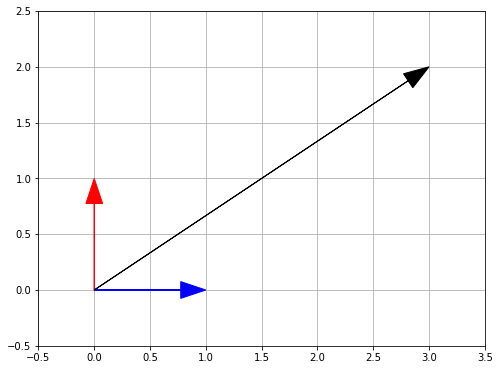
\includegraphics[scale=0.6]{2dvector.png}
\end{frame}

\begin{frame}{Picture in 3D}
  \hspace{-2cm}
  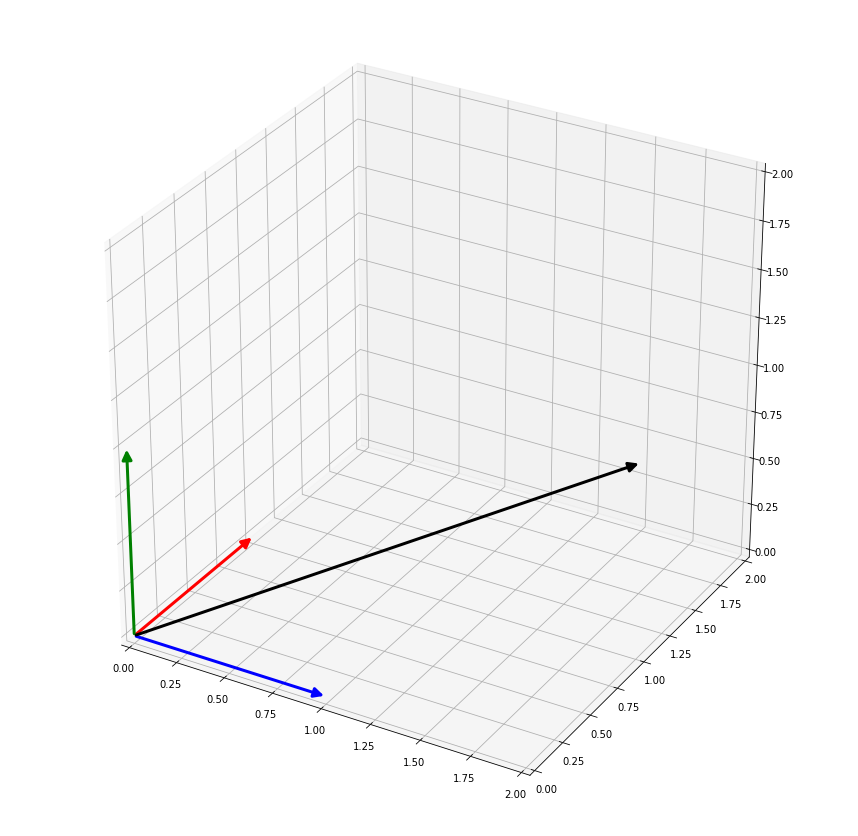
\includegraphics[trim={0 0cm 5cm 13.5cm},clip,scale=0.5]{3dvector.png}
\end{frame}

\begin{frame}{Picture of addition}
  \begin{figure}
    \begin{columns}
      \column{.4\textwidth}
      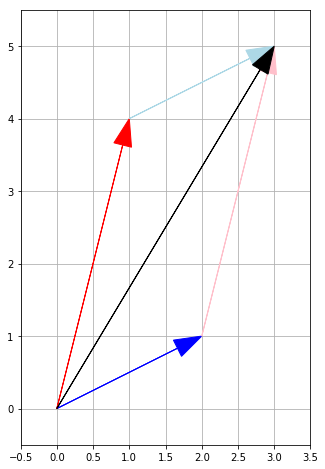
\includegraphics[scale=0.4]{tiptotail.png}
      \column{.5\textwidth}
      \hspace{-2cm}
      \begin{align*}
        \left[
	\begin{array}{c}
          x_1\\
          x_2
	\end{array}
        \right]+\left[
	\begin{array}{c}
          x_3\\
          x_4
	\end{array}
        \right]=
        \left[
	\begin{array}{c}
          x_1+x_3\\
          x_2+x_4
	\end{array}
        \right]
      \end{align*}
    \end{columns}
  \end{figure}
\end{frame}

\begin{frame}{Picture of scalar multiplication}
  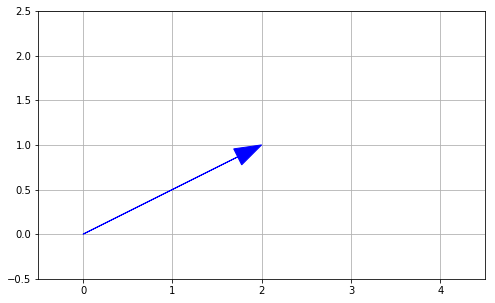
\includegraphics[scale=0.3]{scalarbefore.png}
  \includegraphics[scale=0.3]{scalarafter.png}\\
  \begin{equation*}
    \left[
      \begin{array}{c}
        2\\
        1
      \end{array}
    \right]\mapsto
    2\cdot\left[
      \begin{array}{c}
        2\\
        1
      \end{array}
    \right] = \left[
      \begin{array}{c}
        4\\
        2
      \end{array}
    \right]
  \end{equation*}
  \begin{definition}
    Vectors $A$ and $B$ are \emph{parallel} iff there is some scalar $k$ such that
    \begin{equation*}
      B = kA
    \end{equation*}
  \end{definition}
\end{frame}

\begin{frame}{Notation about base of vector}
  \begin{figure}
    \begin{columns}
      \hspace{-1cm}
      \column{.4\textwidth}
      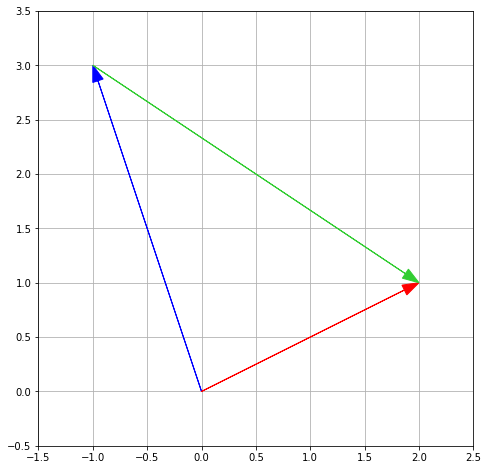
\includegraphics[scale=0.4]{graphicalvector.png}
      \column{0.1\textwidth}
      \column{.4\textwidth}
       \begin{definition}
    We write ${\color{green}\overrightarrow {AB}}$ to denote the vector starting at ${\color{blue}A}$ and ending at ${\color{red}B}$.\\
    Therefore
    \begin{equation*}
      {\color{green}\overrightarrow {AB}} = {\color{red}B}-{\color{blue}A}
    \end{equation*}
  \end{definition}
    \end{columns}
  \end{figure}
\end{frame}

\begin{frame}{Bisection}
  \begin{figure}
    \begin{columns}
      \hspace{-1cm}
      \column{.4\textwidth}
      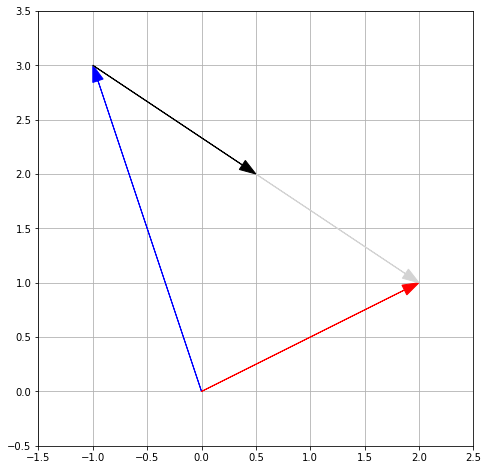
\includegraphics[scale=0.4]{bisection.png}
      \column{0.1\textwidth}
      \column{.4\textwidth}
      \begin{align*}
        &midpoint(A,B)\\
        &= \overrightarrow{0A} + \frac{1}{2}\overrightarrow{AB}\\
                      &= (A-0) + \frac{1}{2}(B-A)\\
                      &= \frac{1}{2}(A+B)
      \end{align*}
    \end{columns}
  \end{figure}
\end{frame}


\begin{frame}
  Questions?
\end{frame}

\begin{frame}{Examples}
  \begin{example}
    Find the point that is midway between
    \begin{equation*}
      \left[
	\begin{array}{c}
          -1\\
          -4\\
          3
	\end{array}
      \right]\text{ and }
      \left[
	\begin{array}{c}
          5\\
          0\\
          -3
	\end{array}
      \right]
    \end{equation*}
  \end{example}
  \begin{example}
    Find the two points trisecting the segment between
    \begin{equation*}
      \left[
	\begin{array}{c}
          2\\
          3\\
          5
	\end{array}
      \right]\text{ and }
      \left[
	\begin{array}{c}
          8\\
          -6\\
          2
	\end{array}
      \right]
    \end{equation*}
  \end{example}
\end{frame}

\begin{frame}{Examples}
  \begin{example}
    Let
    \begin{equation*}
      P = \left[
	\begin{array}{c}
          1\\
          -2\\
          1
	\end{array}
      \right], Q= \left[
	\begin{array}{c}
          -3\\
          0\\
          5
	\end{array}
      \right], X= \left[
	\begin{array}{c}
          2\\
          -1\\
          5
	\end{array}
      \right]\text{ and }Y = \left[
	\begin{array}{c}
          4\\
          -2\\
          3
	\end{array}
      \right]
    \end{equation*}
    Is $\overrightarrow {PQ}$ parallel to $\overrightarrow {XY}$? Is $\overrightarrow {PX}$ parallel to $\overrightarrow {QY}$?
  \end{example}
  \begin{example}
    The diagonals of a parallelogram bisect each other.
  \end{example}
  \begin{example}
    If $ABCD$ is an arbitrary quadrilateral then the midpoints of the four sides form a parallelogram.
  \end{example}
\end{frame}

\section{Equations for lines and planes}

\begin{frame}
  \begin{beamercolorbox}[sep=12pt,center]{part title}
    \usebeamerfont{section title}\insertsection\par
  \end{beamercolorbox}
\end{frame}

\begin{frame}{Two dimensions}
  Given a system of equations
  \begin{align*}
    a_{11}x_1+a_{12}x_2 & = b_1\\
    a_{21}x_1+a_{22}x_2 & = b_2
  \end{align*}
  the solution set could be:-
  \begin{itemize}
  \item empty
  \item a point (a unique solution)
  \item a line (infinitely many solutions)
  \item all of $\mathbb R^2$ (infinitely many solutions)
  \end{itemize}
  \dots and we have to do row reduction to find out which.
\end{frame}

\begin{frame}{Two dimensions}
  The non-trivial situations are:-
  \begin{itemize}
  \item a unique solution
    \begin{equation*}
      \left[
	\begin{array}{c}
          x_1\\
          x_2
	\end{array}
      \right]=
      \left[
	\begin{array}{c}
          c_1\\
          c_2
	\end{array}
      \right]
    \end{equation*}
  \item a single parameter (say $s$)
    \begin{equation*}
      \left[
	\begin{array}{c}
          x_1\\
          x_2
	\end{array}
      \right] = \left[
	\begin{array}{c}
          c_1\\
          c_2
	\end{array}
      \right]+s \left[
	\begin{array}{c}
          d_1\\
          d_2
	\end{array}
      \right]
    \end{equation*}
  \end{itemize}
  \begin{definition}
    A \emph{parametric (vector) equation} describing a line in $\mathbb R^2$ is a vector equation of the form
    \begin{equation*}
      \vec{x} = \vec{c}+s\vec{d}
    \end{equation*}
  \end{definition}
\end{frame}

\begin{frame}{Three dimensions}
  Given a system of equations
  \begin{align*}
    a_{11}x_1+a_{12}x_2+a_{13}x_3 & = b_1\\
    a_{21}x_1+a_{22}x_2+a_{23}x_3 & = b_2\\
    a_{31}x_1+a_{32}x_2+a_{33}x_3 & = b_3
  \end{align*}\vfill
  the solution set could be:-
  \begin{itemize}
  \item empty
  \item a point (a unique solution)
  \item a line (infinitely many solutions)
  \item a plane (infinitely many solutions)
  \item all of $\mathbb R^3$ (infinitely many solutions)
  \end{itemize}
  \dots and we have to do row reduction to find out which.
\end{frame}

\begin{frame}{Three dimensions}
  The non-trivial situations are:-
  \begin{itemize}
  \item a unique solution
  \item a single parameter (say $s$)
    \begin{equation*}
      \left[
	\begin{array}{c}
          x_1\\
          x_2\\
          x_3
	\end{array}
      \right]= \left[
	\begin{array}{c}
          c_1\\
          c_2\\
          c_3
	\end{array}
      \right]+s \left[
	\begin{array}{c}
          d_1\\
          d_2\\
          d_3
	\end{array}
      \right]
    \end{equation*}
     \item two parameters (say $s$ and $t$)
    \begin{equation*}
      \left[
	\begin{array}{c}
          x_1\\
          x_2\\
          x_3
	\end{array}
      \right]= \left[
	\begin{array}{c}
          c_1\\
          c_2\\
          c_3
	\end{array}
      \right]+s \left[
	\begin{array}{c}
          d_1\\
          d_2\\
          d_3
	\end{array}
      \right]+ t \left[
	\begin{array}{c}
          e_1\\
          e_2\\
          e_3
	\end{array}
      \right]
    \end{equation*}
  \end{itemize}
\end{frame}

\begin{frame}{Parametric forms of 3D lines and planes}
  \begin{definition}
    A \emph{parametric (vector) equation} describing a line in $\mathbb R^3$ is a vector equation of the form
    \begin{equation*}
      \vec{x} = \vec{c}+s\vec{d}
    \end{equation*}
    for $\vec{x}$, $\vec{c}$ and $\vec{d}$ in $\mathbb R^3$ and $s$ in $\mathbb R$.
  \end{definition}\vfill
  \begin{definition}
    A \emph{parametric (vector) equation} describing a plane in $\mathbb R^3$ is a vector equation of the form
    \begin{equation*}
      \vec{x} = \vec{c}+s\vec{d}+t\vec{e}
    \end{equation*}
    for $\vec{x}$, $\vec{c}$, $\vec{d}$ and $\vec{e}$ in $\mathbb R^3$ and $s$, $t$ in $\mathbb R$.
  \end{definition}
\end{frame}

\begin{frame}{Properties of parametric form}
  \begin{itemize}
  \item Can immediately see what kind of geometric object it is.\vfill
  \item Often easier to write down.\vfill
  \item The parametric form of a line/plane is {\bf not} unique.
  \end{itemize}
\end{frame}

\begin{frame}{The symmetric form of a line in 3D}
  Sometimes a `half-way' form of the equation of a line in $\mathbb R^3$ is used.\vfill
  \begin{definition}[Symmetric form of equation for line]
    \begin{equation*}
      \frac{x_1+b_1}{a_1} = \frac{x_2+b_2}{a_2} =\frac{x_3+b_3}{a_3}
    \end{equation*}
    where $a_i\neq 0$.
  \end{definition}\vfill
  We can convert this to parametric form immediately by setting all three terms equation to a parameter $s$:
  \begin{align*}
    x_1+b_1&= a_1s\\
    x_2+b_2&= a_2s\\
    x_3+b_3&= a_3s
  \end{align*}
\end{frame}

\begin{frame}
  Questions?
\end{frame}

\begin{frame}{Examples}
  \begin{example}
    Convert the following line into a parametric form
    \begin{equation*}
      \frac{x-2}{3} = \frac{y-1}{2} = z+3
    \end{equation*}
  \end{example}
  \begin{example}
    Write down a parametric equation for the line passing through the points
    \begin{equation*}
      \left[
	\begin{array}{c}
          2\\
          -1\\
          7
	\end{array}
      \right]\text{ and }
      \left[
	\begin{array}{c}
          -3\\
          4\\
          5
	\end{array}
      \right]
    \end{equation*}
  \end{example}
\end{frame}

\begin{frame}{Example}
   \begin{example}
    Write down a parametric equation for the line passing through
    \begin{equation*}
      \left[
	\begin{array}{c}
          4\\
          -7\\
          1
	\end{array}
      \right]
    \end{equation*}
    and parallel to the line
    \begin{equation*}
      \left[
	\begin{array}{c}
          x_1\\
          x_2\\
          x_3
	\end{array}
      \right] = \left[
	\begin{array}{c}
          4\\
          -7\\
          1
	\end{array}
      \right]+t \left[
	\begin{array}{c}
          2\\
          -5\\
          3
	\end{array}
      \right]
    \end{equation*}
  \end{example}
\end{frame}

\begin{frame}{Example}
  \begin{example}
    For the following two lines find the point of intersection.
    \begin{equation*}
      \left[
	\begin{array}{c}
          x_1\\
          x_2\\
          x_3
	\end{array}
      \right] = \left[
	\begin{array}{c}
          3\\
          1\\
          3
	\end{array}
      \right]+ t \left[
	\begin{array}{c}
          1\\
          -2\\
          3
	\end{array}
      \right]\text{ and }
      \left[
	\begin{array}{c}
          x_1\\
          x_2\\
          x_3
	\end{array}
      \right] = \left[
	\begin{array}{c}
          4\\
          6\\
          1
	\end{array}
      \right]+ t \left[
	\begin{array}{c}
          2\\
          3\\
          1
	\end{array}
      \right]
    \end{equation*}
  \end{example}
  \begin{example}
    Write down a system of equations whose solution set is the line
    \begin{equation*}
      \left[
	\begin{array}{c}
          x_1\\
          x_2\\
          x_3
	\end{array}
      \right] = \left[
	\begin{array}{c}
          1\\
          -1\\
          2
	\end{array}
      \right]+s \left[
	\begin{array}{c}
          2\\
          1\\
          3
	\end{array}
      \right]
    \end{equation*}
  \end{example}
\end{frame}

\section{Distance and scalar product}

\begin{frame}
  \begin{beamercolorbox}[sep=12pt,center]{part title}
    \usebeamerfont{section title}\insertsection\par
  \end{beamercolorbox}
\end{frame}

\begin{frame}{Length of a vector}
  \begin{definition}[Two dimensions]
    If $
      \left[
	\begin{array}{c}
          x_1\\
          x_2
	\end{array}
      \right]$
    then $\| \vec{x} \| = \sqrt{x_1^2+x_2^2}$
  \end{definition}
  \begin{definition}[Three dimensions]
    If $\vec{x}=
      \left[
	\begin{array}{c}
          x_1\\
          x_2\\
          x_3
	\end{array}
      \right]$
    then $\| \vec{x} \| = \sqrt{x_1^2+x_2^2+x_3^2}$
  \end{definition}
  \begin{definition}[n dimensions]
    If $\vec{x}=
      \left[
	\begin{array}{c}
          x_1\\
          x_2\\
          \vdots \\
          x_n
	\end{array}
      \right]$
    then $\| \vec{x} \| = \sqrt{x_1^2+x_2^2+\dots +x_n^2}$
  \end{definition}
\end{frame}

\begin{frame}{Distance between two points}
  \begin{definition}[Two dimensions]
    If $\vec{x} =
    \left[
      \begin{array}{c}
        x_1\\
        x_2
      \end{array}
    \right]$ and $\vec{y} =
    \left[
      \begin{array}{c}
        y_1\\
        y_2
      \end{array}
    \right]$
    then $$d(\vec{x}, \vec{y}) = d(0, \vec{y}-\vec{x}) = \sqrt{(x_1-y_1)^2+(x_2-y_2)^2}$$
  \end{definition}
 \begin{definition}[Three dimensions]
    If $\vec{x} =
    \left[
      \begin{array}{c}
        x_1\\
        x_2\\
        x_3
      \end{array}
    \right]$ and $\vec{y} =
    \left[
      \begin{array}{c}
        y_1\\
        y_2\\
        y_3
      \end{array}
    \right]$
    then $$d(\vec{x}, \vec{y}) = d(0, \vec{y}-\vec{x}) = \sqrt{(x_1-y_1)^2+(x_2-y_2)^2+(x_3-y_3)^2}$$
  \end{definition}   
\end{frame}

\begin{frame}{N dimensions and scalar multiplication}
  \begin{definition}[n dimensions]
    If $\vec{x} =
      \left[
	\begin{array}{c}
          x_1\\
          x_2\\
          \dots\\
          x_n
	\end{array}
      \right]$ and $\vec{y} =
      \left[
	\begin{array}{c}
          y_1\\
          y_2\\
          \vdots\\
          y_n
	\end{array}
      \right]$
      then $$d(\vec{x}, \vec{y}) = d(0, \vec{y}-\vec{x}) = \sqrt{(x_1-y_1)^2+(x_2-y_2)^2+\dots +(x_n-y_n)^2}$$
    \end{definition}
    \begin{lemma}[Scalar multiplication]
      If $\vec{v}$ is a non-zero vector and $a$ is a scalar then
      \begin{equation*}
        \|a\vec{v}\| = |a|\|\vec{v}\|
      \end{equation*}
    \end{lemma}
\end{frame}

\begin{frame}{Examples}
  \begin{definition}
    A \emph{unit vector} is a vector with length equal to $1$.
  \end{definition}
  \begin{example}
    The following vectors are unit vectors:-
    \begin{equation*}
      \left[
	\begin{array}{c}
          1\\
          0\\
          0
	\end{array}
      \right],
      \left[
	\begin{array}{c}
          0\\
          1\\
          0
	\end{array}
      \right],
      \left[
	\begin{array}{c}
          0\\
          0\\
          1
	\end{array}
      \right],
      \left[
	\begin{array}{c}
          \sqrt{\frac{1}{2}}\\
          0\\
          - \sqrt{\frac{1}{2}}
	\end{array}
      \right]
    \end{equation*}
  \end{example}
\end{frame}

\begin{frame}{Examples}
  \begin{example}
    Find the distance between
    \begin{equation*}
      \left[
	\begin{array}{c}
          1\\
          -1\\
          3
	\end{array}
      \right]\text{ and }
      \left[
	\begin{array}{c}
          3\\
          1\\
          0
	\end{array}
      \right]
    \end{equation*}
  \end{example}
  \begin{example}
    Find the length of
    \begin{equation*}
      \left[
	\begin{array}{c}
          -3\\
          4
	\end{array}
      \right]\text{ and }
      \left[
	\begin{array}{c}
          3\\
          -1\\
          -2
	\end{array}
      \right]
    \end{equation*}
  \end{example}
\end{frame}

\begin{frame}{Dot product}
  \begin{definition}
    If $\vec{x}$ and $\vec{y}$ are in $\mathbb R^n$ then
    \begin{align*}
      \vec{x}\cdot\vec{y} &= \sum_{i=1}^n x_iy_i\\
                          &= x_1y_1+x_2y_2+\dots +x_ny_n
    \end{align*}
  \end{definition}\vfill
  And so in fact
  \begin{equation*}
    \|\vec{x}\| = \sqrt{\vec{x}\vec{x}}
  \end{equation*}
\end{frame}

\begin{frame}{Examples}
  \begin{example}
    If \begin{equation*}
      u=\left[
	\begin{array}{c}
          1\\
          2\\
          0\\
          -1
	\end{array}
      \right]\text{ and }
      v = \left[
	\begin{array}{c}
          0\\
          1\\
          2\\
          3
	\end{array}
      \right]
    \end{equation*}
    then find $u\cdot v$.
  \end{example}
  \begin{example}
    Find the length of
    \begin{equation*}
      \left[
	\begin{array}{c}
          1\\
          3\\
          5\\
          2
	\end{array}
      \right]
    \end{equation*}
  \end{example}
\end{frame}

\begin{frame}
  Questions?
\end{frame}

\end{document}